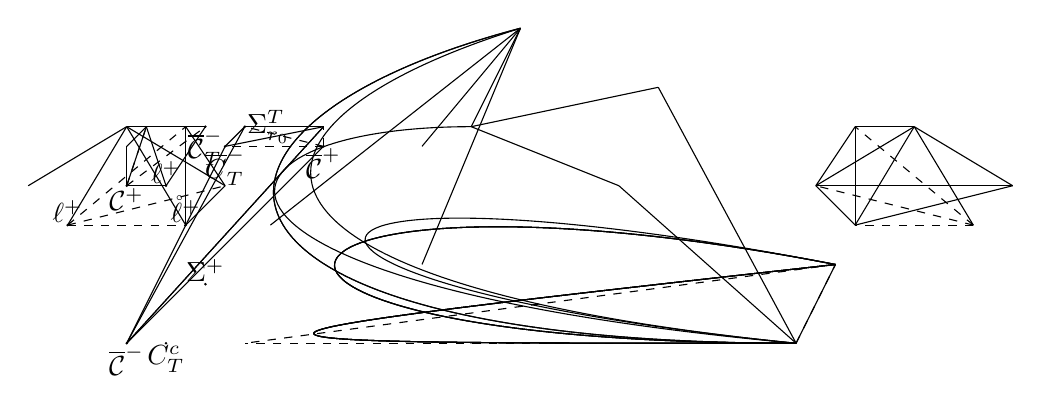
\begin{tikzpicture}[scale=2.5]
\tikzstyle{every node}=[inner sep=0pt]

\coordinate (B) at (-1.27,-1);
\coordinate (C) at (-0.5,-1.2);
\coordinate (D) at (-0.5,-0.6);
\coordinate (A) at (0,0);
\coordinate (E) at (-0.25,-0.5);
\coordinate (F) at (0.5,-0.8);
\coordinate (G) at (0.7,-0.3);
\coordinate (H) at (1.4,-1.6);
\coordinate (I) at (1.6,-1.2);
\coordinate (J) at (1.5,-0.9);
\coordinate (K) at (-1.4,-1.6);

\coordinate (a) at (-2.3,-1);
\coordinate (b) at (-1.7,-1);
\coordinate (c) at (-1.5,-0.8);
\coordinate (d) at (-1.7,-0.5);
\coordinate (e) at (-2,-0.5);
\coordinate (f) at (-2.5,-0.8);

\coordinate (g) at (2.3,-1);
\coordinate (h) at (1.7,-1);
\coordinate (i) at (1.5,-0.8);
\coordinate (j) at (1.7,-0.5);
\coordinate (k) at (2,-0.5);
\coordinate (l) at (2.5,-0.8);

\coordinate (m) at (-2,-0.8);
\coordinate (n) at (-1.8,-0.8);
\coordinate (o) at (-1.6,-0.5);
\coordinate (p) at (-1.9,-0.5);
\coordinate (q) at (-2,-0.6);

\coordinate (r) at (-1,-0.6);
\coordinate (s) at (-1.5,-0.6);
\coordinate (t) at (-1,-0.5);
\coordinate (u) at (-1.4,-0.5);

\coordinate (v) at (-2,-1.6);
\coordinate (w) at (-1.8,-1.6);
\coordinate (x) at (-1.6,-1.3);
\coordinate (y) at (-1.9,-1.3);

\draw[dashed] (H) -- (I);
\draw[dashed] (H) -- (K);
\draw[dashed] (I) -- (K);
\draw (A) -- (B);
\draw (A) -- (C);
\draw (A) -- (D);
\draw (E) -- (A);
\draw (E) -- (F);
\draw (E) -- (G);
\draw (H) -- (G);
\draw (H) -- (F);
\draw (H) -- (I);

\draw[dashed] (a) -- (b);
\draw[dashed] (a) -- (c);
\draw[dashed] (a) -- (d);
\draw (e) -- (a);
\draw (e) -- (f);
\draw (e) -- (d);
\draw (b) -- (e);
\draw (c) -- (e);
\draw (d) -- (e);
\draw (b) -- (c);
\draw (b) -- (d);
\draw (c) -- (d);

\draw[dashed] (g) -- (h);
\draw[dashed] (g) -- (i);
\draw[dashed] (g) -- (j);
\draw (k) -- (g);
\draw (k) -- (l);
\draw (k) -- (j);
\draw (i) -- (k);
\draw (h) -- (k);
\draw (h) -- (l);
\draw (i) -- (l);
\draw (h) -- (i);
\draw (h) -- (j);
\draw (i) -- (j);

\draw[dashed] (m) -- (n);
\draw[dashed] (m) -- (o);
\draw[dashed] (m) -- (p);
\draw (q) -- (m);
\draw (q) -- (p);
\draw (p) -- (o);
\draw (n) -- (o);
\draw (m) -- (n);
\draw (m) -- (p);
\draw (n) -- (p);

\draw[dashed] (r) -- (s);
\draw[dashed] (r) -- (t);
\draw[dashed] (r) -- (u);
\draw (v) -- (r);
\draw (v) -- (t);
\draw (v) -- (u);
\draw (s) -- (v);
\draw (s) -- (u);
\draw (t) -- (v);
\draw (t) -- (u);
\draw (s) -- (t);

\draw (A) .. controls (o) and (x) .. (H);

\draw (A) .. controls (p) and (w) .. (H);
\draw (A) .. controls (p) and (w) .. (H);
\draw (E) .. controls (d) and (y) .. (H);

\draw (H) .. controls (x) and (s) .. (I);

\draw (H) .. controls (w) and (v) .. (I);
\draw (H) .. controls (w) and (v) .. (I);
\draw (H) .. controls (w) and (v) .. (I);
\draw (H) .. controls (v) and (s) .. (I);
\draw (H) .. controls (v) and (s) .. (I);
\draw (H) .. controls (w) and (v) .. (I);
\draw (H) .. controls (v) and (s) .. (I);

\node[circle, fill, inner sep=0pt, minimum size=1pt,label={above:$\ell^+$}] (ell+) at (a) {};
\node[circle, fill, inner sep=0pt, minimum size=1pt,label={below:$\mathcal{C}^+$}] (ell-) at (m) {};
\node[circle, fill, inner sep=0pt, minimum size=1pt,label={above:$\mathring{\ell}^+$}] (ell+m) at (b) {};
\node[circle, fill, inner sep=0pt, minimum size=1pt,label={below:$\overline{\mathcal{C}}^+$}] (ell+-) at (r) {};
\node[circle, fill, inner sep=0pt, minimum size=1pt,label={below:$\overline{\mathcal{C}}^-_{T}$}] (ell+c) at (o) {};
\node[circle, fill, inner sep=0pt, minimum size=1pt,label={right:$\Sigma_{r_{0}}^{T}$}] (ell+c+o) at (u) {};
\node[circle, fill, inner sep=0pt, minimum size=1pt,label={below:$\overline{C}_{T}^{-}$}] (ell+t) at (s) {};
\node[circle, fill, inner sep=0pt, minimum size=1pt,label={above:$\Sigma^{+}$}] (ell+t+) at (x) {};
\node[circle, fill, inner sep=0pt, minimum size=1pt,label={above:$\ell^{+}$}] (ell+m+t) at (n) {};
\node[circle, fill, inner sep=0pt, minimum size=1pt,label={below:$\overline{\mathcal{C}}^{-}$}] (ell+t-t) at (v) {};
\node[circle, fill, inner sep=0pt, minimum size=1pt,label={below:$C^{c}_{T}$}] (ell+t-t+c) at (w) {};

\end{tikzpicture}